\documentclass{atlasnote} 

%\documentclass[usetikz]{atlasnote} % the 'usetikz' option loads tikz.sty in the proper place, 
                                   % avoiding conflicts with graphicx.sty.
                                   % Don't know what tikz.st is? Just ignore this line! :-)

%\documentclass[coverpage]{atlasnote} % the 'coverpage' option loads the ATLAS Cover Page package 
                                      % ans makes sure that the cover page is generated before the
                                      % note title page. Make sure that the latest version of
                                      % of 'atlascover.sty. is installed on your system!

%\usepackage{graphicx} % This is already loaded by the atlasnote class
                       % Just use it to include your plots!

%\usepackage{atlasphysics} % Contains useful shortcuts. Uncomment to use
                           % See instruction.pdf for details

%%%%%%%%%%%%%%%%%%%%%%%%%%%%%%%%%%%%
%           Title page             % 
%%%%%%%%%%%%%%%%%%%%%%%%%%%%%%%%%%%%

\skipbeforetitle{100pt}

% Title
\title{Rucio: Conceptual Model}

% Author
%if not given, typesets ``The ATLAS collaboration''
%\author{The ATLAS Collaboration}

% if multiple authors/affiliations are needed, use the authblk package
\usepackage{authblk}
\usepackage{booktabs}
\renewcommand\Authands{, } % avoid ``. and'' for last author
\renewcommand\Affilfont{\itshape\small} % affiliation formatting
\newcommand{\code}[1]{\texttt{#1}}

\author[1]{Vincent Garonne}
\author[1]{Mario Lassnig}
\author[1]{Angelos Molfetas}
\author[1]{Martin Barisits}
\author[1]{Thomas Beermann}
\author[1]{Graeme A Stewart}
\author[1]{Armin Nairz}
\author[1]{Luc Goossens}

\affil[1]{PH-ADP-CO, CERN}

% Date: if not given, uses current date
\date{7 December 2011\\ Version 1.1}

% Draft version: if given, adds draft version on front page, a
% 'DRAFT' box on top of each other page, and line numbers to easy
% commenting. Comment or remove in final version.
%\draftversion{0.6}

% Journal: adds a 

% Abstract
\abstracttext{ 

  This document describes the conceptual model of the new version of the
  ATLAS Distributed Data Management (DDM) system, Rucio. We
  describe core concepts of the system and the high level interactions
  between Rucio and its clients.

  The DDM system is designed to allow the ATLAS collaboration to
  manage the large volumes of data, both taken by the detector as well
  as generated or derived, in the ATLAS distributed computing
  system. Rucio supports permissions, accouting and quota on
  its accounts, which can represent an ATLAS user, physics group or
  central activity.  Rucio allows the organisation of files into
  arbitary, overlapping datasets and the setting of selected metadata
  properties on both files and datasets. Replication rules can be set
  that instruct the system how to organise and manage
  replicas. Replication policies can be set, allowing the automatic
  generation of rules based on metadata.
  Rucio can group storage elements by the setting
  of common properties that can be specified as part of a replication
  rule. Rucio manages ATLAS accessible storage elements by moving
  required files to them and deleting unnecessary files from them.

}

%%%%%%%%%%%%%%%%%%%%%%%%%%%%%%%%%%%%
%            Content               % 
%%%%%%%%%%%%%%%%%%%%%%%%%%%%%%%%%%%%

\begin{document}

% Test of tikz.sty loadin in atlasnote.cls. Use 'usetkiz' option in documentclass declaration:
% e.g. \documentclass[usetikz]{atlasnote}
% \input{tikz-test}

\section{Introduction}


In this document we describe the conceptual model of the new version
of ATLAS Distributed Data Management (DDM) system: codename Rucio.
We introduce the core concepts Rucio uses to manage accounts, files,
datasets and storage systems. A high level description of how users
interact with the system is given where appropriate.

\section{Rucio account}
\label{overview_Rucio_account::doc}\label{overview_Rucio_account:rucio-account}

A Rucio account is the unit of assigning privileges in Rucio. It can
represent individual users (like \mbox{lgoossen}, graemes, vgaronne, \dots), a
group of users (like bphys, higgs, susy, \dots) or an organised
production activity for the whole ATLAS collaboration (prod,
tzero, \dots). A Rucio account is identified by a string.

Rucio actions are always conducted by a Rucio account. Each account
has a namespace identifier called \emph{scope} that is included in every
name assigned to a collection of data created by that account (see
\S\ref{overview_Dataset:dataset-file-identifiers-and-scope}). By default, Rucio accounts can only create identifiers
in their own scope and not in any other.

A Rucio user is identified by their credentials, like X509 certificate,
username/password, or token. Credentials can map to one or more
accounts (N:M mapping). The Rucio authentication system checks if the
used credentials are authorised to use the supplied Rucio account.
The figure below gives an example of the mapping between credentials
and Rucio accounts:

{\hfill\scalebox{0.800000}{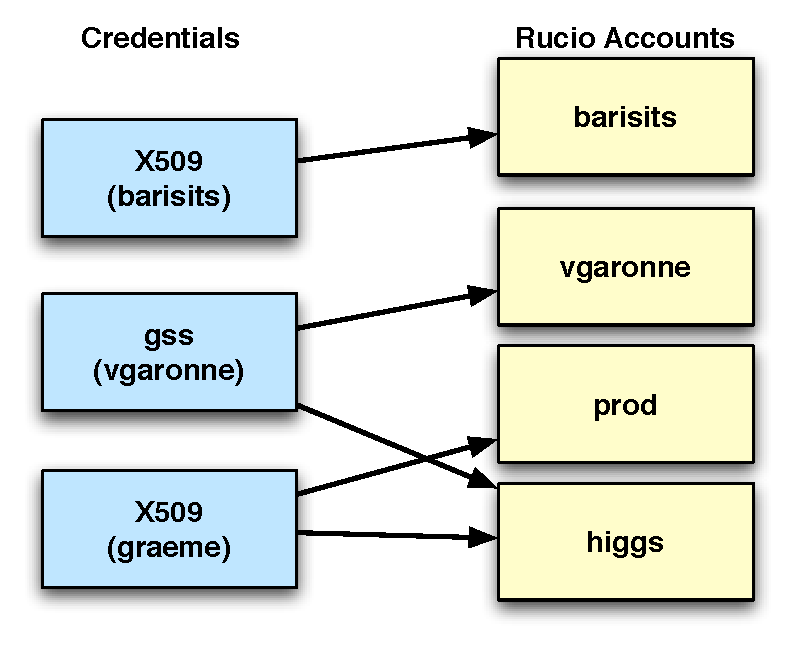
\includegraphics{accounts.pdf}}\hfill}

\newpage

\section{Datasets and files}
\label{overview_Dataset::doc}\label{overview_Dataset:dataset}
ATLAS naturally has a large amount of data, which is physically stored
in files. The actual distribution of the data over files is mostly
incidental. The data consists usually, but not exclusively, of
persistent C++ objects associated with physics events.  Physicists
need to be able to identify and operate on any arbitrary subset of
this data: a dataset.  Hence, a dataset might be a single file or
multiple files, but either case this dataset unit is that on
which most users will act most of the time.

Datasets may be overlapping in the sense that a subset of data, i.e.,
a single file or more files, can be part of multiple datasets.

New datasets can be defined based on the contents of existing
datasets. In particular, it is possible to aggregate the contents of
two or more datasets into a new one by taking the set union of their
respective contents. While successive aggregations will implicitly
create an aggregation hierarchy, this is not reflected in the naming
of the datasets. Instead Rucio will merely record in the dataset
metadata that it was created by performing such a union. Otherwise the
dataset will be identical to one created by simple enumeration of the
resulting contents, i.e., the corresponding files.

The most common aggregation scheme in ATLAS is hierarchical, e.g., run datasets
aggregated into sub-periods, sub-periods into periods, periods into
a year of data. However, Rucio also will support horizontal
aggregation of files between any datasets.


\subsection{Dataset/file identifiers and scope}
\label{overview_Dataset:dataset-file-identifiers-and-scope}

To be able to unambiguously refer to a logical file it needs to have
an identifier.  For a logical file this is the Logical File Name (LFN)
which is composed of two strings: the scope identifier and the file
label.  A
single file is a dataset in itself and as such dataset identifiers
follow the same scheme: Each dataset is identified by the Dataset Name (DSN)
 which is composed of the scope identifier and the dataset label.

The scope identifier partitions the dataset name space into several
sub-spaces. The primary use case for this is to have separate scopes
for production and individual users. There is a one to one
relationship between account and scope.  There are no particular
constraints on the strings used for either scope and labels other than
a restricted set of allowed characters. In particular, it is
possible to use Universally Unique Identifiers (UUIDs) as labels.

Datasets/files are uniquely identified over all time. A DSN/LFN once
used to refer to a dataset/file can never be reused to refer to
another dataset/file, not even if the former has become obsolete or
has been deleted from the system.


\subsection{Dataset and file status}

\subsubsection{File status}
\label{sec:file-status}

The following status flags are supported for files:

\begin{itemize}
\item {}
\code{Obsolete}: True/False
\end{itemize}

The obsolete flag indicates a file which, for one reason or another,
should not be used by the collaboration. A file marked as obsolete
will have all replicas removed from the system. Obsolete LFNs are
remembered by the system to prevent accidental reuse in the future.

\begin{itemize}
\item {}
\code{Lost}: True/False
\end{itemize}

The lost flag indicates that although the logical definition of the
file still exists in Rucio, no physical replicas of the file currently
exist. If the file is recovered from outside Rucio this flag can be
changed from True to False.

\subsubsection{Dataset status}
\label{sec:dataset-status}

\label{sec:status}
The dataset status is reflected by a set of attributes. Datasets in
Rucio can have the following attributes:
\begin{itemize}
\item {} 
\code{Open}: True/False

\end{itemize}

A dataset might be a result of more than one computational process,
therefore the definition of a dataset is not an atomic operation and
can even extend over a large amount of time. For this purpose, a
dataset has an open status to publish its availability, i.e., to
reflect that its content is (not) complete. Open datasets cannot be
used in aggregations. When the filling of the dataset is done, its
state changes to closed and cannot thereafter be reopened.
\begin{itemize}
\item {} 
\code{Monotonic}: True/False

\end{itemize}

If the monotonic mode is enabled files cannot be removed from an open
dataset. Once the monotonic flag is set to True it cannot be unset.

\begin{itemize}
\item {} 
\code{Hidden}: True/False

\end{itemize}

Datasets can be hidden so they do not show up in normal listing operations.
\begin{itemize}
\item {} 
\code{Obsolete}: True/False

\end{itemize}

The obsolete status means that a dataset and its definition should not
be used anymore. Obsoleting a dataset does not obsolete its contents
(however, one can instruct Rucio to obsolete all files which are in a
particular dataset).

\begin{itemize}
\item {} 
\code{Complete}: True/False

\end{itemize}

The data a file points to can be temporarily or permanently lost,
e.g., the system has lost all corresponding physical files. This is
reflected in the lost status of the file and by the
complete/incomplete status of all aggregate datasets containing
them. The file content can be recovered and re-injected in the system
causing the corresponding lost and complete/incomplete statuses to be
updated.

Note that Rucio has no concept of dataset versioning. The loss of
files is simply recorded as described above with a single flag, hence
not recording in what order they were lost. Adding further files
requires the definition of a new dataset with a new identifier. The
latter dataset might reflect the relation with the former, but this is
not required.

\subsubsection{Dataset Replication Policy}
\label{sec:datas-repl-policy}

THIS SECTION IS DRAFT FOR DISCUSSION

The question of file distribution in datasets is an important one. If
the file content of datasets is very widely distributed across many
sites this will maximise the availability of CPU resources that can
be used to process this data. If the files are concentrated at one
site this might be optimal for processing which required the use of
many files at the one time (e.g., merging and archiving to
tape). Using the wrong distribution policy will impact on the
efficiency of processing the data.

Therefore Rucio will support a hinting mechanism which will allow
clients to suggest to the system what the optimal distribution across
sites will be. This will influence the way that the system distributes
files when it is satisfying rules (however, the distribution will be
consistent with the rules, e.g., a rule which directs the data to a
specific site will mean that replication policy could not take effect).

It is therefore proposed to support the following flag at the dataset level:

\begin{itemize}
\item {} 
\code{ReplicationPolicy}: RPValue
\end{itemize}

Precise values of RPValue and the effects they will have need to be
discussed. However, it should be possible to concentrate dataset
content at as few sites as possible or to distribute the data as
widely as possible or to adopt some intermediate strategy. 

In any case, given other constraints in the data management system, it
will be very beneficial to overall efficiency if job processing
systems to not rely on 100\% of files being at a specific site, but
will be able to process data at other sites or transfer as needed in
order to complete tasks.


\section{Metadata attributes}
\label{overview_metadata_attributes:metadata-attributes}\label{overview_metadata_attributes::doc}
Metadata associated with a dataset/file is represented using
attribute/value pairs.  The set of available attributes is
restricted. Metadata attributes are classified into four categories:
\begin{enumerate}
\item System-defined attributes: e.g., size, checksum, creationtime,
  modificationtime, status

\item Physics attributes: e.g., number of events, 
  POOL GUID

\item Production attributes: e.g., task
  and job ID that produced the file, processing campaign ID

\item Data management attributes: necessary for the organisation of
  data on the grid (see \S\ref{overview_Replica_management:replica-management})

\end{enumerate}

For datasets, it is possible that the value of a metadata attribute is
a function of the metadata of its constituents, e.g., the total size
is the sum of the sizes of the constituents. In this case it is
obviously not possible to assign a value to it.

When appropriate and requested, Rucio will check metadata values for
validity, rejecting the attempt to set invalid values. This can used
to ensure that, e.g., POOL GUID is unique and that the Job ID is a
positive integer.

Rucio supports searching for files and datasets based on metadata
values. Wildcard queries or range operations will only be supported on
certain metadata fields. e.g., processing tag can be searched using
wildcards, task ID can be searched using range operators, but scope
can only be an exact match.


\section{Rucio Storage Element}
\label{overview_Rucio_Storage_Element:rucio-storage-element}\label{overview_Rucio_Storage_Element::doc}
A Rucio Storage Element (RSE) is a container for physical files. It is
the smallest unit of storage space addressable within Rucio. It has an
unique identifier and a set of meta attributes describing properties
such as supported protocols, e.g., file, https, srm; host/port
address; quality of service; storage type, e.g., disk, tape, \dots;
physical space properties, e.g., used, available, non-pledged; and geographical zone.

Rucio Storage Elements can be grouped in many logical ways, e.g., the
UK RSEs, the Tier-1 RSEs, or the `good' RSEs. One can reference groups of
RSEs by metadata attributes or by explicit enumeration of RSEs.

RSE tags are expanded at transfer time to enumerate target
sites. Post-facto changes to the sites in an RSE tag list will not
affect currently replicated files.


\subsection{Physical File Name}
\label{overview_Rucio_Storage_Element:physical-file-name}
The Physical File Name (PFN) is a fully qualified name identifying a
replica of a file. PFNs may take the form of file names, URIs, or any
other identifier meaningful to a Rucio Storage Element. The mapping
between the LFN and the PFN is a deterministic function which also
takes RSE and protocol into account. It may also consider the
filename, allowing a separation of PFN based on scope, project or
other criteria.

Normally the upload to an RSE and the registration of an additional
replica is a single operation. For trusted users like the Tier-0 and
PanDA production systems, it is possible to register a replica
uploaded independently.


\section{Permission model}
\label{overview_Permission_model:permission-model}\label{overview_Permission_model::doc}
Rucio assigns permissions to accounts. Permissions are boolean flags
designating whether an account may perform a certain action (read,
write, delete) on a resource (RSE, account, replica, etc.).


\section{Replica management}
\label{overview_Replica_management:replica-management}\label{overview_Replica_management::doc}

\subsection{Replication Rules}
\label{sec:replication-rules}

Replica management is based on replication rules defined on datasets.
A replication rule is owned by an account and defines the
minimum number of replicas to be available on a list of RSEs. Accounts
are allowed to set multiple rules\footnote{ The system may reject
  rules if these violate other policies, e.g., a normal ATLAS user
  would not be allowed to set a rule which committed the system to
  generate 5PB of new replicas or to request replicas on an RSE tape
  system.  }.  Rules may optionally have a limited lifetime and can be
added, removed or modified at any time. Rules can also be locked,
which will prevent their modification until an explicit unlock
operation is performed.

An example listing of replication rules is given below:
\begin{enumerate}
\item \code{prod}: 1x replica @ CERN, no lifetime
\item \code{prod}: 1x replica @ T1TAPE, no lifetime, locked
\item \code{higgs}: 2x replica @ GROUPDISK, no lifetime
\item \code{barisits}: 1x replica @ UST2, until 2012-01-01 00:00
\item \code{vgaronne}: 2x replica @ T1, no lifetime
\item \code{graemes}: 1x replica @ GLASGOW, until 2011-12-25 00:00
\end{enumerate}

The Rucio rule engine validates the rules and creates transfer
primitives to fulfil all rules, e.g., transfer some files from RSE A
to RSE B. The rule engine is triggered when a file is created in the
system, when a new rule is added to a dataset or when one explicitly
requests for the rule to be applied on existing data. The rule engine
will only create the minimum set of necessary transfer primitives to
satisfy all rules.

Files inherit all rules from all datasets they are members of. This
allows users of the system to interact at the dataset level and Rucio
will propagate these rules to the appropriate files. The dataset
ReplicationPolicy (see \S\ref{sec:datas-repl-policy}) will affect how
the system groups files in the same dataset across potential RSEs.

Deletion is triggered per RSE when storage policy dictates that space
must be freed. A reaper service will look for replicas on that RSE
that can be deleted without violating any replication rules. The
reaper will use a Least Recently Used (LRU) algorithm to select
replicas for deletion. The reaper service will also immediately delete
all replicas of any file which is declared obsolete.


\subsection{Transfer Primitives}
\label{sec:transfer-primitives}

Accounts can inject transfer primitives directly, e.g.,
transient replicas required for production operations. Notifications
can be provided for the transfer request. All transfer requests are
transient.

The injection of transfer primitives requires a specific privileges to
prevent abuse of this feature.

\subsection{Policies}
\label{sec:policies}

Policies are system entities which generate rules or transfer requests
based on matching particular dataset metadata at registration
time. Polices are owned by an account and can only generate rules for
that account. Policies may have a lifetime, after which they will
expire.

An example of a policy is given below:

\medskip

\begin{tabular}{l p{6cm}}
  \textbf{Attribute} & \textbf{Value} \\\hline
  Owner & tzero \\\hline
  match & project=data11\_7TeV,  dataType=RAW, stream=physics\_* \\\hline
  rule & 1@CERNTAPE, 1 @T1TAPE \\\hline
  lifetime & 2012-01-01 00:00 \\\hline
\end{tabular}

\bigskip
 
Policies can also create transfer primitives, so generate extra copies
of data as it is produced:

\medskip

\begin{tabular}{l p{6cm}}
  \textbf{Attribute} & \textbf{Value} \\\hline
  Owner & prod \\\hline
  match & \sloppy project=mc11\_7TeV, dataType=merge.AOD,
  tag=*(p795$\mid$p796$\mid$p805)*, {ReplicationPolicy}=RPValue \\\hline
  rule & 1@T1DISK, 1@T2DISK \\\hline
  transfer & 1@T1DISK, 2@T2DISK \\\hline
  lifetime & 2011-12-01 00:00  \\\hline
\end{tabular}

\medskip
 
In this case the transfer request is for \emph{extra} copies, in
addition to those set by rules. (This is different behaviour to that
for rules themselves, which are always independent.)

\section{Accounting and quota}
\label{overview_Accounting_and_quota:accounting-and-quota}\label{overview_Accounting_and_quota::doc}
Accounting is the measure of how much resource, e.g., storage, an
account has used as a consequence of its actions. Quota is a policy
limit which the system applies to an account. Quotas will be available
which apply to an account at a specific RSE tag or globally.

For storage accounting, Rucio accounts will only be accounted for the
files they set replication rules on. Accounting is based on the
replicas an account requested, not on the actual amount of physical
replicas in the system. Consequently, it is expected that over-booking
of physical space will be employed as a particular physical replica
may satisfy several replication rules.


\section{Notifications}
\label{overview_Notifications:notifications}\label{overview_Notifications::doc}
External applications can require synchronisation on events relative
to data availability and can subscribe to particular 
events, e.g., dataset state changes. Rucio will then publish a message
to external application when it detects these events.

\section*{Acknowledgments}
\label{Acknowledgments::doc}\label{Acknowledgments:acknowledgments}
We express our gratitude to our ATLAS colleagues for their help and
patience when we explored requirements and use cases, especially:
Markus Elsing, Beate Heinemann, Jamie Boyd, Jonas Strandberg, Solveig Albrand, Torre Wenaus, Rodney
Walker, Tadashi Maeno, Paul Nilsson, Simone Campana, Johannes
Elmsheuser, Daniel Van Der Ster, Junji Tojo, Ikuo Ueda, Borut
Kersevan, Stephane Jezequel and Cedric Serfon.


We would also like to thank Philippe Charpentier, Costin Grigoras,
Simon Metson, Latchezar Betev, and Pablo Saiz for their input and
ideas about the different distributed data management system of each
LHC experiment, and their patience when answering our questions.

\newpage

\label{rucio:appendices}

\section*{Appendix A. Key concepts: Comparison matrix DQ2 vs. Rucio}
\label{Comparison_matrix::doc}\label{Comparison_matrix:key-concepts-comparison-matrix-dq2-vs-rucio}
\begin{tabular}{l l p{5cm} }
\toprule
\textbf{
Features
} & \textbf{
DQ2
} & \textbf{
Rucio
}\\
\midrule

File identifier
 & 
GUID/LFN (Basename)
 & 
Scope + Label name
\\

Dataset identifier
 & 
DUID/DSN
 & 
Scope + Label name
\\

Versioning
 & 
Yes
 & 
No
\\

Namespace
 & 
Global/Flat
 & 
Scoped
\\

Unique PFN
 & 
No
 & 
Yes
\\

Overlapping dataset
 & 
Yes
 & 
Yes
\\

Storage Element Groups
 & 
No
 & 
Yes
\\

Storage Element Tagging
 & 
No
 & 
Yes
\\

Quota support
 & 
Group
 & 
Account (Group/User)
\\

Dataset Replica completeness
 & 
Yes
 & 
No
\\

Dataset Distribution Policy
&
Only complete at site
&
Flexible
\\

Replica Lifetime
&
Yes
&
No
\\

Metadata namespace/support
 & 
System defined, Data placement
 & 
System defined, Physics, Production, Analysis, Data placement
\\

Data discovery unit
 & 
Pattern
 & 
Metadata
\\

Data operation unit
 & 
Dataset
 & 
Dataset, File
\\

Multiple replica ownership
 & 
No
 & 
Yes
\\

Dynamic placement
 & 
No
 & 
Yes
\\

Replication rule support
 & 
No
 & 
Yes
\\

Hidden data
 & 
Yes
 & 
Yes
\\

Reuse of dataset name
 & 
No
 & 
No (but possibility to resuscitate dataset)
\\

Notifications
 & 
Yes
 & 
Yes
\\

Fine-grained accounting
 & 
Partially
 & 
Yes
\\
\bottomrule
\end{tabular}


\newpage
\section*{Appendix B. Acronyms and Abbreviations}
\label{Acronyms_and_Abbreviations:acronyms-and-abbreviations}\label{Acronyms_and_Abbreviations::doc}\begin{description}
\item[{LFN}] \leavevmode
Logical File Name.

\item[{LRU}] \leavevmode
Least Recently Used.

\item[{DSN}] \leavevmode
Dataset Name.

\item[{PFN}] \leavevmode
Physical File Name.

\item[{RSE}] \leavevmode
Rucio Storage Element.

\item[{UUID}] \leavevmode
Universal Unique Identifier.

\end{description}




\end{document}
